\documentclass[acmsmall,review,anonymous]{acmart}

%\settopmatter{printfolios=true,printccs=false,printacmref=false}


\overfullrule=3mm
\citestyle{acmauthoryear}
%\setcitestyle{round}

\usepackage{multirow}

\usepackage{alltt}
% \usepackage{amssymb}
\usepackage{calc}
\usepackage[noabbrev]{cleveref}
\usepackage{colortbl}
\usepackage{listings}
\usepackage{mathpartir}
\usepackage{graphicx}
\usepackage{pifont}
\usepackage{subcaption}
\usepackage{tikz}
\usepackage{wrapfig}
\usepackage{xcolor}
\usetikzlibrary{arrows.meta}
\usetikzlibrary{positioning}
\usetikzlibrary{shapes.geometric}

\usepackage{moreverb}

%%%%%%%%%%%%%%%%%%%%%%%%%%%%%%%%%%%%%%%%%%%%%%%%%%%%%%%%%%%%%%%%%%%%%%%%%%%%%%%%%%%%%%%%%%%%
%%%%%%%%%%%%%%%%%%%%%%%%%%%%%%%%%%%%%%%%%%%%%%%%%%%%%%%%%%%%%%%%%%%%%%%%%%%%%%%%%%%%%%%%%%%%
%%%%%%%%%%%%%%%%%%%%%%%%%%%%%%           PREAMBLE       %%%%%%%%%%%%%%%%%%%%%%%%%%%%%%%%%%%% 
%%%%%%%%%%%%%%%%%%%%%%%%%%%%%%%%%%%%%%%%%%%%%%%%%%%%%%%%%%%%%%%%%%%%%%%%%%%%%%%%%%%%%%%%%%%%
%%%%%%%%%%%%%%%%%%%%%%%%%%%%%%%%%%%%%%%%%%%%%%%%%%%%%%%%%%%%%%%%%%%%%%%%%%%%%%%%%%%%%%%%%%%%

\usepackage{tcolorbox}

%%%%%%%%%%%%%%%%%%%%%%%%%%%%%%%%%%%%%%%%%%%%%%%%%%%%%%%%%%%%%%%%%%%%%%%%%%%%%%%%%%%%%%%%%%%%
%%%%%%%%%%%%%%%%%%%%%%%%%%%%%%%%%%%%%%%%%%%%%%%%%%%%%%%%%%%%%%%%%%%%%%%%%%%%%%%%%%%%%%%%%%%%
%%%%%%%%%%%%%%%%%%%%%%%%%%%%%%%%%%%%%%%%%%%%%%%%%%%%%%%%%%%%%%%%%%%%%%%%%%%%%%%%%%%%%%%%%%%%

\newcommand{\set}[1]{\ensuremath{\bar{#1}}}

\newcommand{\size}[1]{\ensuremath{\mid #1 \mid}}

\newcommand{\setsize}[1]{\left|#1\right|}



%% %%%%%%%%%%%%%%%%%%%%%%%%%%%%%%%%%%%%%%%%%%%%%%%%%%%%%%%%%%%%%%%%%%%%%%%%%%%%%
%% for leaving margin notes in the paper write
%% \yourinitials{...} 

\def\notes#1{\expandafter\def\csname#1\endcsname##1{\marginpar{\textcolor{red}{\raggedright\tiny $\bullet$ #1 says: ##1}}}}
\notes{mf}
\notes{cd}
\notes{bg}


%% %%%%%%%%%%%%%%%%%%%%%%%%%%%%%%%%%%%%%%%%%%%%%%%%%%%%%%%%%%%%%%%%%%%%%%%%%%%%%


%% strategies

\newcommand{\sfont}[1]{\textit{#1}}

\newcommand{\featkw}{\sfont{boundary}}

\newcommand{\statkw}{\sfont{statistical}}

\newcommand{\totalkw}{\sfont{total}}

\newcommand{\selfkw}{\sfont{self}}

\newcommand{\stat}[1]{\sfont{\statkw(#1)}}

\newcommand{\statself}{\sfont{\stat{\selfkw}}}
\newcommand{\stattotal}{\sfont{\stat{\totalkw}}}

\newcommand{\optkw}{\sfont{optimistic}}

\newcommand{\conkw}{\sfont{conservative}}

\newcommand{\costkw}{\sfont{cost\textsf{-}aware}}

\newcommand{\confkw}{\sfont{configuration\textsf{-}aware}}

\newcommand{\randkw}{\sfont{null}}

\newcommand{\togglekw}{\sfont{toggling}} % either-or ... gotta rebuild plots

\newcommand{\agnostickw}{\sfont{profiler\textsf{-}agnostic}}

\newcommand{\strategy}[2]{#1~#2}

\newcommand{\strategyext}[3]{#1~\strategy{#2}{#3}}


\newcommand{\featopt}{\strategy{\featkw}{\optkw}}
\newcommand{\statselfopt}{\strategy{\statself}{\optkw}}
\newcommand{\stattotalopt}{\strategy{\stattotal}{\optkw}}

\newcommand{\featcon}{\strategy{\featkw}{\conkw}}
\newcommand{\statselfcon}{\strategy{\statself}{\conkw}}
\newcommand{\stattotalcon}{\strategy{\stattotal}{\conkw}}

\def\costoptkw{\strategy{\costkw}{\optkw}}

\newcommand{\featcostopt}{\strategyext{\featkw}{\costkw}{\optkw}}
\newcommand{\statselfcostopt}{\strategyext{\statself}{\costkw}{\optkw}}
\newcommand{\stattotalcostopt}{\strategyext{\stattotal}{\costkw}{\optkw}}

\def\costconkw{\strategy{\costkw}{\conkw}}

\newcommand{\featcostcon}{\strategyext{\featkw}{\costkw}{\conkw}}
\newcommand{\statselfcostcon}{\strategyext{\statself}{\costkw}{\conkw}}
\newcommand{\stattotalcostcon}{\strategyext{\stattotal}{\costkw}{\conkw}}

\newcommand{\featconf}{\strategy{\featkw}{\confkw}}
\newcommand{\statselfconf}{\strategy{\statself}{\confkw}}
\newcommand{\stattotalconf}{\strategy{\stattotal}{\confkw}}

\newcommand{\randomopt}{\strategy{\randkw}{\optkw}}
\newcommand{\randomcon}{\strategy{\randkw}{\conkw}}

\newcommand{\toggle}{\togglekw}

%% types

\newcommand{\type}{\ensuremath{t}}

\newcommand{\deep}{\ensuremath{deep}}

\newcommand{\shallow}{\ensuremath{shallow}}


%% program, components, strategy

\newcommand{\program}{\ensuremath{P}}


\newcommand{\component}{\ensuremath{c}}

\newcommand{\strategyvar}{\ensuremath{S}}


%% lattice

\newcommand{\latticeL}{\mathcal{L}}

\newcommand{\lattice}[1]{\ensuremath{\latticeL\llbracket#1\rrbracket}}

\newcommand{\standardlattice}{\lattice{\system}{\kmap}}

\newcommand{\conf}{\ensuremath{k}}

\newcommand{\metric}{\ensuremath{\leq_{\latticeL}^{X}}}


\newcommand{\modem}{\ensuremath{M}}
\newcommand{\mode}[1]{\ensuremath{\modem\llbracket#1\rrbracket}}

\newcommand{\orderkw}{\ensuremath{<}} 
\newcommand{\ordered}[2]{\ensuremath{#1 \orderkw #2}}

\newcommand{\orderqkw}{\ensuremath{\leqslant}} 
\newcommand{\orderqed}[2]{\ensuremath{#1 \orderqkw #2}}

%% performance


\newcommand{\slowdownkw}{\ensuremath{slowdown}}
\newcommand{\slowdown}[2]{\ensuremath{\slowdownkw(#1,#2)}}

\newcommand{\takikawa}{\ensuremath{T}}



\begin{document}

\title{How Profilers Can Help Navigate Type Migration}

\author{Ben Greenman}
\orcid{0000-0001-7078-9287}
\affiliation{%
  \institution{PLT @ Brown University}
  \city{Providence}
  \state{Rhode Island}
  \country{USA}
}
\email{benjaminlgreenman@gmail.com}

\author{Matthias Felleisen}
\orcid{0000-0001-6678-1004}
\affiliation{%
  \institution{PLT @ Northeastern University}
  \city{Boston}
  \state{Massachusetts}
  \country{USA}
}
\email{matthias@ccs.neu.edu}

\author{Christos Dimoulas}
\orcid{0000-0002-9338-7034}
\affiliation{%
  \institution{PLT @ Northwestern University}
  \city{Evanston}
  \state{Illinois}
  \country{USA}
}
\email{chrdimo@northwestern.edu}

%\renewcommand{\shortauthors}{...}

%%
%% The abstract is a short summary of the work to be presented in the
%% article.
%% -----------------------------------------------------------------------------

\begin{abstract}
Sound migratory typing promises a safe and smooth refactoring of untyped code
bases to typed ones. Over the past few years, it has become clear that enforcing
soundness with run-time checks imposes a large performance overhead, too large
to deploy many of the partially typed programs.  Finding a smooth path from a
configuration with performance problems to an acceptable one is difficult due to
the exponential size of the migration lattice. The process requires an effective
interpretation of feedback from profiling tools. This paper reports on the
results of a rational-programmer experiment on tens of thousands of
performance-debugging scenarios. These results shed light on how well particular
uses of profiling tools work for these performance-debugging issues. At the same
time, the experiment once again confirms the usefulness of the
rational-programmer method.
\end{abstract}

%%
%% The code below is generated by the tool at http://dl.acm.org/ccs.cfm.
%% Please copy and paste the code instead of the example below.

\begin{CCSXML}
<ccs2012>
<concept>
<concept_id>10011007.10011006.10011039.10011311</concept_id>
<concept_desc>Software and its engineering~Semantics</concept_desc>
<concept_significance>500</concept_significance>
</concept>
<concept>
<concept_id>10011007.10011006.10011008.10011024.10011032</concept_id>
<concept_desc>Software and its engineering~Constraints</concept_desc>
<concept_significance>100</concept_significance>
</concept>
<concept>
<concept_id>10011007.10011006.10011008.10011009.10011012</concept_id>
<concept_desc>Software and its engineering~Functional languages</concept_desc>
<concept_significance>100</concept_significance>
</concept>
</ccs2012>
\end{CCSXML}

\ccsdesc[500]{Software and its engineering~Semantics}
\ccsdesc[100]{Software and its engineering~Constraints}
\ccsdesc[100]{Software and its engineering~Functional languages}

\newcommand{\code}[1]{\texttt{#1}}
\newcommand{\cmod}[1]{\parbox[c][1.4ex]{2em}{\code{#1}}}
\newcommand{\stdrkt}{\code{v8.6.0.2 [cs]}}
\newcommand{\bmname}[1]{\textsf{#1}}
\newcommand{\totalnumconfigs}{116,154}
\newcommand{\totalnummeasurements}{1277694}
%% 2023-03-22 bg: configs + runs ignoring quadT
\newcommand{\machinename}[1]{\texttt{#1}}
\newcommand{\commitname}[2]{\texttt{#1}}
\newcommand{\gcell}[1]{\cellcolor{green!20}#1}
\newcommand{\wcell}[1]{\cellcolor{black!05}#1}
\newcommand{\ycell}[1]{\cellcolor{yellow!18}#1}
\newcommand{\ocell}[1]{\cellcolor{orange!29}#1}
\newcommand{\rcell}[1]{\cellcolor{red!30}#1}
\newcommand{\tcell}[1]{\cellcolor{black!10}#1}

\keywords{gradual typing, migratory typing, rational programmer, profiling}

\maketitle

%% -----------------------------------------------------------------------------

\section{Type Migration as a Navigation Problem}
\label{sec:intro}
%% -----------------------------------------------------------------------------

Sound migratory typing promises a safe and smooth refactoring path from an
untyped code base to a typed one~\cite{tf-dls-2006, tfffgksst-snapl-2017}. It
realizes the safe part with the compilation of types to run-time checks that
guarantee type-level integrity of each mixed-typed program configuration.
Unfortunately, these run-time checks impose a large performance
overhead~\cite{gtnffvf-jfp-2019}, making the path anything but smooth. While
this problem is particularly stringent for deep run-time
checks~\cite{tf-dls-2006, st-sfp-2006},\footnote{\citet{kas-pldi-2019}
demonstrate a low overhead for a lambda-calculus-sized programming
language. This research is yet to be applied to a language that supports more
than a set of select micro-benchmarks.}  it also applies to shallow run-time
checking~\cite{gm-pepm-2018}.

\citet{g-thesis-2020,g-deep-shallow} presents evidence that deep and shallow
checks actually come with complementary strengths and weaknesses. Deep checking
imposes a steep cost yet enables type-driven optimizations that off-set
some---and sometimes more than all---of the cost as more type annotations are
added. By contrast, shallow checking is a pay-as-you-go scheme; a developer pays
only for the type annotations added and the worst-case cost seems to be capped
at an order-of-magnitude. Hence, Greenman argues that developers should, in
principle, be able to mix and match deep and shallow checking to get the
best-possible type checking benefits with a tolerable performance penalty.
Greenman has implemented this idea for Typed Racket; programmers can
switch from deep to shallow and back with a one-line edit.  Initial empirical data
is promising: with a mixture of checks developers can avoid migration paths that
result in unacceptable slowdowns with either deep or shallow checks alone.
However, the mixture of deep and shallow checks makes it even more difficult to
find a smooth migration path. With a purely shallow or purely deep type checking
scheme, developers have to pick from $2^N$ configurations of a program with $N$
components that can be typed or untyped. In a context with both deep and shallow
checking, the size of the configurations space goes to $3^N$.

This situation raises the question:
\begin{quote} \em
 how to navigate the migration lattice of a code base while keeping
 the performance penalty from run-time checks at acceptable levels.
\end{quote}  
Like all performance problems, this situation calls for the use of profiling
tools. But, this conventional response merely refines the above question in two
ways, namely,
\begin{itemize} \em

\item how to use feedback from various profiling tools to guide a navigation; and

\item how well feedback helps find a path from a bad configuration to one with
 tolerable performance.

\end{itemize}   

Such questions call for an empirical investigation, though using human
developers for a large number of performance problems is too costly and too
error-prone. Instead, this paper reports on the results of a \emph{rational
programmer} experiment~\cite{lksfd-popl-2020,lgfd-icfp-2021}. The method employs algorithmic
abstractions, dubbed rational programmers, that reify a falsifiable hypothesis
about various ways of using profiling tools and interpreting their feedback.
These algorithmic abstractions are then applied to a diverse population of
problematic performance scenarios. A rational-programmer experiment simulates the
satisficing behavior of developers in a large number of performance-debugging
situations and thus enables a systematic comparison of different ways
programmers can interpret profiler feedback.

In short, this paper makes two contributions:
\begin{itemize}

\item At the object level, the results of the rational programmer experiment
 provide guidance to developers about how to best use the feedback from
 profilers during type migration.

\item At the meta level, the application of the rational programmer method to
 the performance problems of type migration provides one more piece of evidence
 about its usefulness. 
    
\end{itemize}    
The remainder of the paper is organized as follows.  Section~\ref{sec:seascape}
uses an example to explain the problem in concrete terms. Section~\ref{sec:ideas}
introduces the rational programmer method and shows how its use can help evaluate the
effectiveness of a performance-debugging strategy systematically. Section
\ref{sec:experiment} lays out the details of how these ideas translate to a
large-scale quantitative experiment.  Section~\ref{sec:results} presents the data
collected from the experiment.
\Cref{sec:discussion} extracts lessons
for developers and researchers.  Section~\ref{sec:related} places this work in
the context of prior research.
\Cref{sec:conclusion} puts this work in
perspective with respect to future research.
\section{Navigating the Deeps and Shallows via Profiling Tools}
\label{sec:seascape}
%% -----------------------------------------------------------------------------

Over the years, developers have created many large systems in untyped languages.
In the meantime, language implementors have created gradually typed siblings of
these languages.  Since developers tend to enjoy the benefits of type-based IDE
support and a blessing from the type checker, they are likely to add new
components in the typed sibling language. Alternatively, when a developer is
confronted with debugging an untyped component, it takes a large mental effort
to reconstruct the informal types of fields, functions, and methods, and to make
this effort pay off, it is best to turn the informal types into formal
annotations. In either case, the result is a mixed-typed software system with
boundaries between typed and untyped components.

In a sound gradual language, these boundaries impose a performance penalty.  Languages can
enforce sound types with deep or shallow checks. A deep check means that types are
translated to higher-order contracts~\cite{ff-icfp-2002,tf-dls-2006,st-sfp-2006}.
Higher-order contracts impose many kinds of performance penalties: they check all
compound values when they cross a boundary; they wrap all higher-order values with
proxies to delay checks; and such proxies also raise memory consumption. By
contrast, a shallow check means that types are enforced only with tag-level
assertions and only inside of typed components~\cite{vss-popl-2017,
vksb-dls-2014}. Each check is inexpensive, but the more type annotations a
programmer adds, the more run-time checks the compiler inserts for typed
components. As a result, the performance penalty can become prohibitive in
either case. If so, the developer faces a performance-debugging scenario.

To make this concrete, consider the \bmname{fsm} program from the GTP benchmark
suite~\cite{gtnffvf-jfp-2019}. The program is the creation of \citet{fsm},
economists interested in simulating an economy of agents with deterministic
strategies. Figure~\ref{f:fsm-code:a} shows the outline of the four-module
program: \code{auto} implements state machines; \code{pop} coordinates among
machines; \code{main} drives the simulation and permits users to set a number of
simulation parameters; and \code{util} provides helper functions.  Focusing on
just the modules of this program suffices because in Typed Racket, the migration
granularity is a module.

The variant of \bmname{fsm} on the left of figure~\ref{f:fsm-code:a} is untyped.
If a developer adds deep types to the \code{main} module, performance is
significantly degraded. The mixed-typed variant runs almost three times
($3x$) slower than the untyped one.  Switching to shallow types does not remedy
the situation. 

%% 3x not terrible compared to prior work [CITE popl], but still bad.
%% Collapsible helps fsm but not in this particular config & not in fsmoo.

At this point, the question is how to recover the performance of the untyped
variant. The first option is to roll back the addition of types, but developers
prefer typed code and dislike undoing the effort of adding types. The second one
is to add (deep or shallow) types to a random module connected to \code{main}---following a
``hunch'' like programmers sometimes do---but doing so can easily make things
worse. For example, if the choice were the \code{auto} module with shallow
types, then performance would degrade further (a 9x slowdown, to be
precise). Finally, adding deep types to every module is the option that is almost
always guaranteed to fix the situation, and in this context, it would produce a
performance improvement over the untyped variant.  However, such a choice
represents a heavy migration effort, which a programmer who simply
wishes to fix \code{main} and deploy again may be reluctant to invest.

%% -----------------------------------------------------------------------------
%% fsm next steps:
%% 1100 => 2.87x
%% 2100 => 9.04x
%% 2200 => 9.06x
%% 1200 => 2.88x

\begin{figure}[htb]\centering
  %% profiler output: data/example-output-fsm/*

  \begin{subfigure}[t]{\columnwidth}\centering
    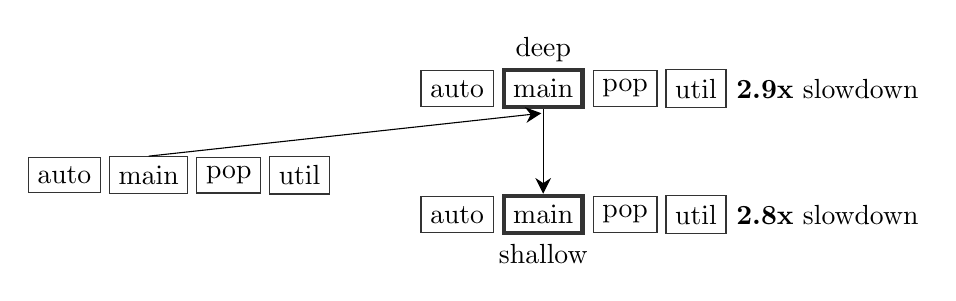
\begin{tikzpicture}
      \node (1) [draw=black!80] {\cmod{util}};
      \node (1c) [draw=black!80,left=of 1.west,xshift=9mm] {\cmod{pop}};
      \node (1b) [draw=black!80,left=of 1c.west,xshift=9mm] {\cmod{main}};
      \node (1a) [draw=black!80,left=of 1b.west,xshift=9mm] {\cmod{auto}};
%      \node (0) [above of=1a,yshift=-2mm] {Program: \bmname{fsm}};

      \node (2) [above of=1,yshift=1mm,xshift=2cm,draw=black!80] {\cmod{auto}};
      \node (2a) [draw=black!80,line width=0.6mm,right=of 2.east,xshift=-9mm] {\cmod{main}};
      \node (2tgt) [below of=2a,yshift=7mm,xshift=1mm] {};
      \node (2b) [draw=black!80,right=of 2a.east,xshift=-9mm] {\cmod{pop}};
      \node (2c) [draw=black!80,right=of 2b.east,xshift=-9mm] {\cmod{util}};
      \node (22) [right=of 2c.east,xshift=-10mm] {\textbf{2.9x} slowdown};
%      \node (24) [above of = 22,yshift=-6mm] {Deep types};

      \node (3) [below of=2,yshift=-6mm,draw=black!80] {\cmod{auto}};
      \node (3a) [draw=black!80,line width=0.6mm,right=of 3.east,xshift=-9mm] {\cmod{main}};
      \node (3b) [draw=black!80,right=of 3a.east,xshift=-9mm] {\cmod{pop}};
      \node (3c) [draw=black!80,right=of 3b.east,xshift=-9mm] {\cmod{util}};
      \node (33) [right=of 3c.east,xshift=-10mm] {\textbf{2.8x} slowdown};
%      \node (34) [above of = 33,yshift=-6mm] {Shallow types};

      \node (dlbl) [above of=2a,yshift=-5mm] {deep};
      \node (slbl) [below of=3a,yshift=5mm] {shallow};

      \draw[-{Stealth[length=2mm,width=2mm]}] (1b.north) -- (2tgt);
      \draw[-{Stealth[length=2mm,width=2mm]}] (2a.south) -- (3a.north);

    \end{tikzpicture}

    \caption{Adding deep or shallow types to one \bmname{fsm} module degrades performance} \label{f:fsm-code:a}
  \end{subfigure}

  \bigskip

  \begin{subfigure}[t]{0.53\columnwidth}
%%-------------------------------------------------
%% [1] 1192(100.0%)   0(0.0%)  body of ....
%%                              body of ....
%%-------------------------------------------------
%%                              profile-thunk [5]
%% [6] 1192(100.0%)   0(0.0%)  ??? profile-lib
%%                              body of "main" [7]
%%                              t [8]
%%                              body of ....
%%-------------------------------------------------

    \footnotesize
    \begin{boxedverbatim}
  Total cpu time observed: 1192ms (out of 1236ms)
  Number of samples taken: 23 (once every 52ms)

=================================================
                              Caller
 Idx   Total       Self      Name+src
       ms(pct)     ms(pct)    Callee
=================================================
                              ??? [12]
                              evolve [17]
[17]  818(68.6%)    0(0.0%)  evolve main
                              evolve [17]
                              shuffle-vector [19]
                              death-birth [18]
                              ??? [20]
-------------------------------------------------
                              match-up* [22]
                              shuffle-vector [19]
[24]  152(12.7%)  152(12.7%) contract-wrapper
-------------------------------------------------
    \end{boxedverbatim}
    \caption{Statistical profiler output for the top-right variant} \label{f:fsm-code:statistical}
  \end{subfigure}~\begin{subfigure}[t]{0.44\columnwidth}
    \footnotesize
    \begin{boxedverbatim}
cpu time: 984 real time: 984 gc time: 155
Running time is 18.17% contracts
253/1390 ms

(interface:death-birth pop main)
  142 ms
  (->* ((cons/c (vectorof automaton?)
                (vectorof automaton?))
        any/c)
       (#:random any/c)
       (cons/c (vectorof automaton?)
               (vectorof automaton?)))
(interface:match-up* pop main)
  81.5 ms
  (-> ....)
(interface:population-payoffs pop main)
  29 ms
  (-> ....)


    \end{boxedverbatim}
    \caption{Boundary profiler output for the same variant} \label{f:fsm-code:boundary}
  \end{subfigure}

  \caption{Profiling during type migration} \label{f:fsm-code}
\end{figure}
%% -----------------------------------------------------------------------------

Still, the idea to continue the migration effort is a good one, because we know
that there are a fair number of well-performing
variants as well as badly-performing ones. The question is how to make progress.

Clearly, informed feedback is needed for a solution that recovers performance
with a reasonable effort. Lacking alternatives, a developer might reach for a
profiling tool to determine the source of the performance
degradation. Fortunately Racket comes with two such tools: 
\begin{itemize}

\item a traditional \emph{statistical profiler}, which identifies the time spent
 in modules; and

\item a \emph{boundary profiler}, which  attributes the cost of types-as-contracts to
 specific module boundaries~\cite{astavf-feature-prf, staaf-feature-prf}.
 
\end{itemize}
Both tools are potentially useful due to the mechanics of deep and shallow types.
In Racket, deep types compile to contracts at module
boundaries~\cite{tf-popl-2008}, so the boundary profiler should identify the
expensive ones.  Shallow types compile to assertions within typed
code~\cite{glfd-pj-2022}, meaning the statistical profiler may uncover their
cost.

The bottom half of \cref{f:fsm-code} shows the output of the statistical
profiler and the boundary profiler for the top-right (deep) variant of \bmname{fsm} in
figure~\ref{f:fsm-code:a}, respectively.

\paragraph{Statistical profiler} \Cref{f:fsm-code:statistical} lists two
rows from the statistical profiler; the full output has 28 rows.  The
first row, labeled \code{[17]}, covers a large percentage (\code{68\%}) of the
total running time, and it refers to a function named \code{evolve}, which is
defined in the \code{main} module. The line suggests that calls from
\code{evolve} to other modules account for a high percentage of the total cost.
The second row, labeled \code{[24]}, says that a contract wrapper accounts for a
significant chunk (\code{12.7\%}) of the running time.  The caller of this
contract, from row \code{[19]} (not shown) is the function \code{shuffle-vector}
from the \code{pop} module.  Putting these clues together, the profiling output
identifies the boundary between \code{main} and \code{pop} as a significant
contributor to the overall cost. 

This conclusion, however, is one of many that could be drawn from the full
statistical profiler output.  The \code{util} module also appears in the output,
and may be more of a performance problem that the \code{pop} module.  Equally
unclear is whether the column labeled \code{Total} is a better guide than
the column labeled \code{Self} or vice versa.  High
total times point to a context that dominates the expensive parts.  High self
times point to expensive parts, but these costs might be from the actual
computation rather than the overhead of type-checking.

\paragraph{Boundary profiler} \Cref{f:fsm-code:boundary} shows nearly-complete
output from the boundary profiler; only two contracts are omitted.  This
profiling output attributes \code{18.17\%} of the total running time to
contracts, specifically, to the contracts on the three functions whose names are
prefixed with \code{interface:}. This output indicates that the contracts are
wrapped on untyped functions that flow into typed code. The modules involved are
\code{main} and \code{pop}.  Since \code{pop} is the untyped one, the hint is to
type it.

Adding types to \code{pop} does improve performance. Concretely, this variant
suffers from a 1.2x slowdown.  If this overhead is acceptable, the developer is
done; otherwise, it might be necessary to continue with another round of
profiling, searching, and typing.


\paragraph{Summary}

At first glance, the effort of eliminating a performance problem seems
straightforward. Several factors complicate the search, however. First, a
programmer has two typing options not just one. Second, for programs with more
than four modules, the output of profiling tools is much more complex;
identifying the next step in such a context is hard. Finally, adding types to the
profiler-identified module may degrade the performance even more, in which case
the programmer may wish to give up. In sum, navigating a migration lattice with
$3^N$ program configuration is a non-trivial effort, and developers deserve to
know how well profiling tools help with this effort. 


\section{A Rational Approach to Navigation}
\label{sec:ideas}
%% -----------------------------------------------------------------------------

When a developer confronts a newly created performance-debugging scenario, one
possible response is to erase the types and to return to the {\em status quo
ante\/}.  Another one is to use a profiling tool to reduce the overhead. If the
second alternative is chosen, the question arises:
\begin{quote} \em

 how the developer should modify the program to obtain tolerable performance.
 
\end{quote}   
The type-migration lattice suggests two answers.  The developer should either
add types to an untyped component or toggle the run-time checks for a typed one
from deep to shallow or vice versa.  After all, the fully typed program with
deep types is often faster than its untyped
counterpart; if so, migration is guaranteed to eliminate any performance
problem sooner or later.

Deciding which of the alternatives to pursue in a given situation poses the
follow-up question:
\begin{quote} \em

how a developer should interpret the feedback from a profiling tool to
choose a modification.

\end{quote}   
Operationally, this question asks how the feedback is turned into a
modification at each step of the performance-debugging process.

Unlike the first question, this second one does not have a simple answer.  At
each step, the developer has to choose a specific component to modify.  The
sequence of choices should result in a migratory path along which performance
improves. Assuming that the chosen profiling tool identifies components that
contribute to the performance degradation, it is rational for the programmer to
rely on this feedback to rank the components and to identify the
highest-priority one for adding types or for toggling its run-time checking.

Stepping back, these two insights suggest an experiment to determine which
profiling tool combined with which strategy helps developers make progress with
performance debugging. For this experiment, the developer must choose a
profiling tool---statistical or boundary---and a modification strategy.
To determine the best combination(s) means to have developers work through a
large number of performance-debugging scenarios. The result should help guide a
developer with toggling or adding types to resolve performance-related
problems during type migration.

Since it is obviously impossible to ask a developer to work through thousands of
performance-debugging scenarios, an alternative experimental method is needed.
The rational-programmer method provides a framework for conducting such
large-scale systematic examinations.

The method is inspired by the well-established idea of rationality in
economics~\cite{mill1874essays, henrich2001search}.  In more detail, a (bounded)
rational agent is a mathematical model of an economic actor. Essentially, it
abstracts an actual economic actor to an entity that, in any given
transaction-scenario, acts strategically to maximize some kind of benefit.  Of
course, the strategy cannot be fully rational given the bounded nature of human
beings and the limits in available information. Hence, investigations in modern
times use rational agents that are bounded; they do not make maximally optimal
choices and settle for \emph{satisficing}~\cite{hs:satisfice} their goal.

Analogously, a rational programmer is a model of a developer who aims to resolve
a problem in a work context---a scenario---with bounded
resources. Specifically, it is an algorithm that implements a developer's
bounded strategy for \emph{satisficing} its goal. Using such algorithms, it is
possible to inspect the effectiveness of an approach on a large quantity of
scenarios. In turn, comparing the results of such runs for different modes
can inform human programmers about the success chances of a strategy
in some specific work context. In short, a rational-programmer evaluation yields
insights into the pragmatic value of work strategies. So far, the rational
programmer has been used to evaluate strategies for debugging logical mistakes;
this paper presents the first application to a performance problem. 

\medskip

%% -----------------------------------------------------------------------------
\paragraph{A sketch of a rational-programmer experiment for performance
debugging migratory typing overhead problems.}  In the context of profiler-guided
type migration, a rational programmer consists of two interacting pieces.  The
first is strategy-agnostic; it consumes a program, measures its running time,
and if the performance is tolerable, stops. Otherwise it faces a
performance-debugging scenario and asks for guidance from the second,
strategy-specific piece. This second piece profiles the given program---using
the boundary profiler or the statistical profiler---and analyzes the
profiling information. Based on this analysis, it modifies the program by adding
types to some untyped component to eliminate a boundary or by toggling the run-time
enforcement of types for a typed component. This modified version is handed back
to the first piece of the rational programmer. 

In fact, as the discussion implies, there are numerous versions of the rational
programmer that differ in their strategy-specific piece. Each such version,
dubbed a \emph{mode}, can be applied to realistic performance-debugging
scenarios and use its specific strategy to resolve the problems.  For any given
scenario, the mode either succeeds in eliminating the performance overhead or
fails.
Failure may occur either because the strategy cannot propose a program modification, or
because the chosen modification worsens the performance of the program.

Data about successes and failures for different modes can shed light on the
usefulness of one profiling strategy compared to another. Intuitively, the
success rate of a mode (in)validates the hypothesis that its strategy has
pragmatic value. Similarly, the comparison of the success rates of two different
modes on the same scenario clarifies the relative pragmatic value of the
two. Collecting the data necessary for drawing reliable conclusions calls for an
experiment that pits a spread of strategies against each other on a large and
diverse set of performance-debugging scenarios. Of course, the experiment may
also reveal shortcomings of the profiling approach altogether---which then
demands additional research from tool creators. 
\section{From a Rational Approach to a Rational Programmer Experiment}
\label{sec:experiment}

%% -----------------------------------------------------------------------------

Turning the sketch from section~\ref{sec:ideas} into a large-scale automated
experiment requires formal descriptions: the modes of the rational programmer;
the strategies that create modes from the rational programmer; and the notion of
debugging scenario. A strategy component identifies the next migration step.
Every mode of the rational programmer recognizes whether a given program is a
performance-debugging scenario; if so, it applies a strategy to the profiler
feedback and migrates the program---which should yield a performant program or
another performance-debugging scenario.  The preceding section also implies that
a strategy's response is one of three possibilities: (1) to add types and to
specify their enforcement regime (deep, shallow); (2) to toggle from one regime
to another; or (3) to fail to act. Hence it is possible to specify strategies
independently of the scenarios per se. Equipped with formal descriptions, it is
possible to turn the generic research question of the introduction into
questions with a quantitative nature.

This section provides the required formal descriptions.
Section~\ref{subsec:strategies} presents the profiling strategies.
Section~\ref{subsec:lattice} characterizes the starting navigation points
(performance-debugging scenarios)
and how a type-based migration is a
path through a lattice of program configurations. Using these definitions, It
also lays out the criteria for successes and failures. Finally,
section~\ref{subsec:questions} formalizes the precise experimental questions and
the experimental procedure that answers them.

%% -----------------------------------------------------------------------------

\subsection{The Profiling Strategies}
\label{subsec:strategies}
%% -----------------------------------------------------------------------------
Every program \program{} is a collection of interacting components $\component$.
Some components have deep types, some shallow ones, and some
are untyped. Independently of their types, a component $\component{}_1$, may
import another component $\component{}_2$, which establishes a \emph{boundary}
between them, across which they exchange values at run time. Depending on the
kind of types at the two sides of the boundary, a value exchange can trigger
run-time checks, which may degrade the performance.

A profiling strategy should thus aim to eliminate the most costly boundaries in
a program. In formal terms, a profiling strategy is a function that consumes a
program \program{} and, after determining its profile, returns a set of pairs
$(\component{}, \type{})$. Here \type{} is either \deep{} or \shallow{}. Each
such pair prescribes a modification of \program{}. For instance, if a strategy
returns the singleton set with the pair $(c, \deep)$, then the strategy directs
its rational-programmer mode to equip component $c$ with types (if necessary)
and set its enforcement strategy to deep; if $c$ is typed, it just requests
toggling from shallow to deep.  If a strategy's result is the empty set, it
cannot figure out how to proceed.

%% -----------------------------------------------------------------------------

\def\with{with {\em total\/} in place of {\em self\/}}

\begin{figure}[htb]

  \newcommand{\desc}[1]{\parbox[t]{24em}{#1\\[-2mm]}}
  
  \def\desca{\desc{Uses the boundary profiler to identify the most
    expensive boundary in the given program. Then it directs the mode to equip
    both sides of the target boundary with deep types.}}

  \def\descb{\desc{Like \featopt{} but with shallow types for both
    sides of the target boundary.}}

  \def\descc{\desc{Uses the statistical profiler to identify the component
    $\component{}_1$ with the highest self time in the given program that has a
    boundary with at least one component $\component{}_2$ that has stricter
    types than $\component{}_1$.  Then it picks the component $\component{}_2$
    that has the highest self time, and directs the mode to equip both
    $\component{}_1$ and $\component{}_2$ with deep types.}}

  \def\descd{\desc{Like \statselfopt{} \with}}

  \def\desce{\desc{Like \statselfopt{}, with shallow types for $\component{}_1$, $\component{}_2$}}

  \def\descf{\desc{Like \statselfcon{} with {\em total\/} in place of {\em self\/}}}

 \begin{tabular}{l l l}
    {\bf Profiler} & {\bf Response} & {\bf Description} \\ \hline
    %%%%%%%%%%%%%%%%%%%%%%%%%%%%%%%%%%%%%%%%%%%%%%%%%%%%%%%%%%%%%%%%
    \multirow[b]{2}[+5]{*}{{\em boundary\/}} & 
        \optkw{}          &   \desca          \\ \relax
     &	\conkw{}          &   \descb          \\ \hline

    \multirow[b]{2}[+7]{*}{{\em statistical\/} ({\em self\/})} &
	\optkw{}      &   \descc          \\ \relax
     &	\conkw{}      &   \desce          \\ \hline

    \multirow{2}{*}{{\em statistical\/} ({\em total\/})} & 
	\conkw{}     &   \descf           \\ \relax
     &	\optkw{}     &   \descd           % \\ \relax
 \end{tabular}

 
  \caption{The Basic Strategies of the Experiment and their Descriptions}
  \label{f:bstrategies}
\end{figure}
%% -----------------------------------------------------------------------------

\paragraph{Basic strategies.}  Figure~\ref{f:bstrategies} describes six basic
 strategies that rational programmers may use. 

At the first level, the basic strategies differ in whether they employ the
 \featkw{} or the \statkw{} profiler to profile the given program.  Those that
 use the first kind of profiler can directly identify the most costly boundary
 in \program{} and suggest a modification of either of the two components.
 Those that use the second cannot directly identify a boundary.  Instead they
 focus on the most costly component $\component{}_1$ in terms of either
 \selfkw{} or \totalkw{} time.  From there, they pick one of the boundaries
 between $\component{}_1$ and any of the components that it depends on or that
 depend on it. The goal is to find a boundary between $\component{}_1$ and a
 component $\component{}_2$ where $\component{}_2$ has \emph{stricter} types
 than $\component{}_1$, because in this case, the interactions across the
 boundary are likely to generate costly run-time type checks. Here, deep is
 stricter than shallow, and shallow is stricter than untyped. If the strategy
 cannot identify such a boundary, it moves on to the next costly component
 (again in terms of either \selfkw{} or \totalkw{} time). Once it eventually
 identifies a target boundary, the strategy decides how to migrate the
 two components.

At the second level, basic strategies differ in how they migrate the two sides
 of their target boundary. Strategies that are \optkw{} turn the types at either
 side of the boundary to deep. After all, when two components with deep types
 interact, no checks take place and, better still, deep enforcement may even
 enable type-driven compiler optimizations for the two components.  Hence, such
 a migration may eliminate the cost of the boundary entirely.  Experience shows,
 however, that switching to deep type enforcement for a component may cause a
 ripple effect. The new deeply enforced types may increase the cost of other
 boundaries between (one of) the two components and a third one. By contrast,
 \conkw{} strategies choose shallow enforcement of types for both sides of the
 target boundary. The rationale behind this choice is that, if both sides of a
 boundary have shallow types, the interactions across the boundary cost less
 than if only one is deep and, at the same time, unlike with \optkw{}
 strategies, there is no risk of a ripple effect.

%% -----------------------------------------------------------------------------
\begin{figure}[b]
 
  \newcommand{\desc}[1]{\parbox[t]{19.5em}{#1\\[-2mm]}}
 
  \def\desca{\desc{Splits the boundaries in the given program to those between
    typed components and the rest.  Delegates to \featopt{} to produce a
    modification for the given program, but rank boundaries in the first group
    higher than those in the second group while determining the most expensive
    boundary.}}

  \def\descb{\desc{Like \featcostopt{} but it delegates to \featcon{}.}}

  \def\descc{\desc{Separates the typed components that have boundaries with
    other typed components from the rest of the components in the given
    program. Delegates to \statselfopt{} to produce a modification for the given
    program, but rank boundaries between components in the first group higher
    than the rest while determining the most expensive boundary.}}

   \def\descd{\desc{Like \statselfcostopt{} but it delegates to \stattotalopt{}.}}

   \def\desce{\desc{Like \statselfcostopt{} but it delegates to \statselfcon{}.}}

   \def\descf{\desc{Like \statselfcostopt{} but it delegates to \stattotalcon{}.}}

   \def\descg{\desc{If the number of typed components in the given program is
     above a threshold $N$, it delegates to \featopt{}. Otherwise, it delegates
     to \featcon{}.}}

   \def\desch{\desc{Like \featconf{}; it delegates to \statselfopt{}
     or \statselfcon{} instead.}}

  \def\descj{\desc{Like \featconf{}; it delegates to \stattotalopt{}
     or \stattotalcon{} instead.}}

 \begin{tabular}{l l l}
    {\bf Profiler} & {\bf Response} & {\bf Description}  \\ \hline
    %%%%%%%%%%%%%%%%%%%%%%%%%%%%%%%%%%%%%%%%%%%%%%%%%%%%%%%%%%%%%%%%
    \multirow[b]{2}[+19]{*}{{\em boundary\/}} & 
    \costoptkw{}      &   \desca           \\ \relax
    & \costconkw{}      &   \descb           \\ \relax
    & \confkw{}         &   \descg           \\ \hline

    \multirow[b]{2}[+17]{*}{{\em statistical\/} ({\em self\/})} &
    \costoptkw{}   &   \descc           \\ \relax
    & \costconkw{}   &   \desce           \\ \relax
    & \confkw{}      &   \desch           \\ \hline

    \multirow{2}[+17]{*}{{\em statistical\/} ({\em total\/})} & 
    \costoptkw{} &   \descd           \\ \relax
    & \costconkw{} &   \descf           \\ \relax
    & \confkw{}    &   \descj           % \\ \relax

 \end{tabular}

 
  \caption{The Composite Strategies of the Experiment and their Descriptions}
  \label{f:cstrategies}
\end{figure}
%% -----------------------------------------------------------------------------

\paragraph{Composite strategies.} While the basic strategies ignore the cost of
 adding types to an untyped components, developers do not. Adding types to an
 entire module in Typed Racket may require a significant effort. Hence, the
 experiment includes composite strategies that account for this cost.

Figure~\ref{f:cstrategies} lists these composite strategies. In addition to the
 performance cost reported in the profile, the \costkw{} strategies rank the
 cost of boundaries in terms of the labor needed to equip the two components
 with types.  They give priority to those boundaries that involve components
 that are already typed.  For those, migration just means toggling their type
 enforcement regime, which is essentially no labor.  As pointed out, ripple
 effects also factor into the decisions that strategies have to make. The
 \confkw{} strategies decide whether to be \optkw{} or \conkw{} based on how
 many components are already typed.  When most components are untyped, the risk
 of a ripple effect outweighs the benefits of an \optkw{} strategy. Hence
 strategies favor a \conkw{} approach for sparsely typed programs and an
 \optkw{} strategy for densely typed ones.

\paragraph{Baseline Strategies} An experiment must include baselines, i.e., the
 building block for a null hypothesis. In terms of strategies, the experiment
 needs a \agnostickw{} strategy.  If this \agnostickw{} strategy is less
 successful in eliminating performance problems than the profiling ones, then
 the feedback from the profiler plays a meaningful role; otherwise, the
 experiment is meaningless.

The results presented in the next section include two modes using
 \agnostickw{} strategies. The first one, \randkw{}, aims to invalidate the null
 hypothesis with random choices. Specifically, it picks a random boundary with
 types of different strictness and suggests to modify the two sides of the
 target boundary in either an \optkw{} or a \conkw{} manner.  The second
 \agnostickw{} strategy, \togglekw{}, is due to~\citet{g-deep-shallow}. It
 serves as a point of comparison with Greenman's results, which do not rely on
 profiling information. If the given program uses a mixture of shallow and deep
 enforcement, the strategy directs its rational-programmer mode to equip all
 typed components with deep enforcement. If all components already use deep, it
 instructs the mode to toggle the enforcement to shallow.
\subsection{Migration Lattices and their Navigation}
\label{subsec:lattice}
\newcommand{\gtpurl}{\url{https://docs.racket-lang.org/gtp-benchmarks/index.html}}
%% -----------------------------------------------------------------------------

Gradual type migration is an open and challenging problem for realistic
programs~\cite{rch:in-out-infer-gt, km:ts-type-evo,
mp:gt-decidable, ccew:gt-migrate, gc:gt-infer,
cagg-solver-based-migration,clps-popl-2020,js-infer,ruby-static-infer,unif-infer,
msi:gt-infer-hm,dyn-infer-ruby,profile-guided-typing,jstrace,gen-ts-decl,
lambdanet,nl2ptype,learn-types-big-data,ml-ts}. For
any untped component, a migrating programmer has to choose among several
practical type annotations and often among an infinite number of theoretical
ones. But, to make a rational-programmer experiment computationally feasible, it
is necessary to avoid this dimension.

Fortunately, the construction of the corpus of scenarios from a carefully
selected set of suitable seed programs can solve the problem. For instance, the
established GTP benchmarks~\cite{gtnffvf-jfp-2019}\footnote{\gtpurl{}} are
representative of the programming styles in the Racket world, and they come with
well-chosen type annotations for all their components.  Hence, the migration
lattices can be pre-constructed for all benchmark programs.  It is thus possible
to start a rational programmer mode from any performance-debugging scenario in
this lattice---a program with intolerable performance---and make it use the
known types of the components to chart a path through the program's migration
lattice.

A rational-programmer mode thus combines a strategy \strategyvar{} with a
function that picks points from the migration lattice. That is, the mode
$\mode{\strategyvar{}}$ is a partial function from a program $\program{}_0$ to a
program $\program{}_n$. To get from $\program{}_0$ to $\program{}_n$,
$\mode{\strategyvar{}}$ iterates \strategyvar{} on its input and applies its
recommendations to obtain the next $\program{}_i$.  In other words, $\mode{\strategyvar{}}$
constructs a \emph{migration path}, a sequence of programs ${\program{}_0},
\ldots, {\program{}_n}$ from a migration lattice. If \strategyvar{} cannot make
a recommendation at any point in this lattice, $\mode{\strategyvar{}}$ does not
produce a result. The following definitions translate these points into rigorous
language. 

\paragraph{The Migration Lattice.}  All programs $\program{}_i$ are nodes in the
\emph{migration lattice} \lattice{\program{}_u} where ${\program{}_u}$, is like
${\program{}_i}$ but all its components are untyped. The bottom element of
\lattice{\program{}_u} is ${\program{}_u}$; its top elements are
${\program{}_u}$'s fully typed versions $\program{}_t$ (with some combination of
deep and shallow). In between these extreme points are all the remaining
\emph{configurations} of $\program{}_u$. The $3^N$ configurations of
\lattice{\program{}_u} are ordered: $\ordered{\program{}_i}{\program{}_j}$ iff
$\program{}_j$ has at least one component that is untyped in
$\program{}_j$. Hence the lattice is organized in \emph{levels} of incomparable
configurations, each of which lacks types for the same components but differs
from others in the choice of enforcement regime for one (or more) of its typed
components.  $\orderqed{\program{}_i}{\program{}_j}$ denotes that either
$\program{}_i$ and $\program{}_j$ are at the same level or $\program{}_i$ is at
some level below $\program{}_j$.

A migration path corresponds to a collection of configurations $\program{}_i$,
$0 \leq i < n$, such that $\orderqed{\program{}_i}{\program{}_{i+1}}$. In fact,
either $\program{}_i$ and $\program{}_{i+1}$ are at the same level or they are
at two neighboring ones.  This statement is the formal equivalent to the
description from the preceding section that strategies either add types to a
single previously untyped component or toggle the type enforcement of existing
typed components.\footnote{None of the strategies modifies a boundary where both
side are untyped. Such boundaries are invisible to the boundary
profiler, and the strategies that use the statistical one explicitly filter them
out. Ditto for the profiler-agnostic ones.}  In other words, a migration path is
a weakly ascending chain in
\lattice{\program{}_u}.

%% MF: I think this is obvious. We can discuss if you think not. 

% This last observation is key for the implementation of the rational-programmer
% experiment. If for each $\program{}_u$ in the experiment, one of its fully type
% versions $\program{}_t$ is also available, then the construction of
% \lattice{\program{}_u} is automatic, and as a result, so are the modifications
% that the strategies produce. Therefore, given implementations of the strategies
% and a collection of seed programs with both untyped and fully typed versions,
% the rational-programmer experiment reduces to a fully automated push-button
% process that asks all modes of the rational programmer to construct a migration
% path starting at the same configurations of
% \lattice{\program{}_u}, and compares their successes. 

\paragraph{Performance-debugging scenarios and success criteria.} Completing the
formal description of the experiments demands answers to two more questions.

The first concerns the selection of the starting points for the modes of the
rational programmer, i.e., the \emph{performance-debugging scenarios}.  The
answer is that every configuration $\program$ that exhibits performance
degradation compared to $\program{}_u$ above a certain threshold is an
interesting starting point for a rational-programmer exploration.

\begin{quote} \em

Given a migration lattice \lattice{\program{}_u},
a \emph{performance-debugging scenario} is a configuration $\program$ in \lattice{\program{}_u} 
iff
\slowdown{\program}{\program{}_u} > \takikawa{},\\
 where \slowdown{\program}{\program{}_u} is the ratio of the performance of \program{} over the performance of $\program{}_u$,\\ 
 and $\takikawa{}$ is a constant that signifies the maximum acceptable performance degradation.
\end{quote}

The second question is about differentiating successful from failing migrations.
In this case, there are two answers. Strictly speaking, performance should
always improve, otherwise the programmer may not wish to invest any more effort
into migration.  In the worst case, performance might stay the same for a few
migration steps, before it becomes tolerable.

\begin{quote} \em

A migration path ${\program{}_0} \ldots {\program{}_n}$ in a lattice \lattice{\program{}_u}
is \emph{strictly successful}
iff
\begin{enumerate}
  \item $\program{}_0$ is a performance-debugging scenario,
  \item $\slowdown{\program{}_n}{\program{}_u} \leq \takikawa{}$, and 
  \item for all $0 \leq i < n$, $\slowdown{\program{}_{i+1}}{\program{}_{i}} \leq 1$.
 \end{enumerate} 
\end{quote}
The construction of a strictly successful migration path requires a strategy
that suggests modifications that monotonically improve the performance of  a
program en route to making it performant.

The alternative to strict success is to represent a programmer who tolerates
occasional setbacks. Accepting that a migration path may come with $k$ setbacks,
a $k$-loose success relaxes the requirement for monotonicity $k$ times.

\begin{quote} \em

A migration path ${\program{}_0} \ldots {\program{}_n}$ in a
lattice \lattice{\program{}_u} is \emph{$k$-loosely successful}
iff 
\begin{enumerate}
  \item  $\program{}_0$ is a performance-debugging scenario,
  \item $\slowdown{\program{}_n}{\program{}_u} \leq \takikawa{}$  
  \item
      for all $0 \leq i < n$ with at most $k$ exceptions,
      $\slowdown{\program{}_{i+1}}{\program{}_{i}} \leq 1$
      \subitem equivalently: $k \geq |\{ \slowdown{\program{}_{i+1}}{\program{}_{i}} > 1 \mid 0 \leq i < n\}|$
  \end{enumerate} 
\end{quote}
The construction of a $k$-loose successful migration path allows a strategy to
temporarily worsen performance. The constant $k$ is an
upper bound on the number of missteps.

A patient programmer may wish to relax this constraint even more.

\begin{quote} \em
A migration path ${\program{}_0} \ldots {\program{}_n}$ is $N$-loosely successful if 
  \begin{enumerate}
  \item  $\program{}_0$ is a performance-debugging scenario,
  \item $\slowdown{\program{}_n}{\program{}_u} \leq \takikawa{}$  
  \end{enumerate}
\end{quote}

\subsection{The Experimental Questions}
\label{subsec:questions}
%% -----------------------------------------------------------------------------

Equipped with rigorous definitions, it is possible to formulate the research
questions precisely:
\begin{description}

\item[$Q_X$] How successful is a strategy $X$ with the elimination of
  performance overhead?

\item[$Q_{X/Y}$] Is strategy $X$ more successful than strategy $Y$ in this
  context?
  
\end{description}

Answering $Q_X$ boils down to determining the success and failures of
$\mode{X}$, the rational-programmer mode of $X$ for all performance-debugging
scenarios in all available lattices. If, for a large number of scenarios,
$\mode{X}$ charts migration paths that are strictly successful, the answer is
positive. Essentially, the large number of scenarios is evidence that when a
rational programmer reacts to profiler feedback following $X$, it is likely to
succeed with tuning the performance of mixed-typed code. Notably, the above
description uses the strict notion of success, which sets a high bar.
Hence, the rational programmer not only manages to tune performance at
a tolerable level but each suggestion of its strategy brings the rational
programmer closer to its target. Swapping the notion of strict success for
$k$-loose success relaxes this high standard, and offers answers to $Q_X$ when
allowing for some bounded flexibility in how well the intermediate suggestions
of $X$ help the rational programmer. For completeness, the next section also
reports the data collected for the notion of $N$-loose success.

While an answer to $Q_X$ constitutes an evaluation of a strategy $X$ for
interpreting profiler feedback in absolute terms, an answer to $Q_{X/Y}$ is
about the relative value of $X$ versus some other strategy
$Y$. Answering this second question asks whether the proportion of scenarios
where $\mode{X}$ charts a successful path but $\mode{Y}$ does not is higher that
the proportion of scenarios where $\mode{Y}$ charts a successful path but
$\mode{X}$ does not. Of course, the answer may not be clear cut as $X$ and $Y$
may perform equally well in most scenarios or may have complementary success
records. But, relaxing the notion of success by different factors $k$ may
help distinguish $X$ and $Y$ based on the quality of the feedback they produce.

Importantly, when $Y$ is the $\randkw{}$ strategy and the answer to
$Q_X/\randkw$ is positive, then the experiment invalidates its null-hypothesis.
Put differently, the success of $X$ is not due to sheer luck but the rational
use of profiler feedback.

Summing up, the process for answering $Q_X$ and $Q_{X/Y}$ rests on the following
experimental plan:
\begin{enumerate}

\item Create a large and diverse corpus of performance-debugging scenarios.

\item Calculate the migration paths for each mode of the rational programmer for
  each scenario.

\item Compute and compare the successes and failures of the modes.

\end{enumerate}



\section{The Results of the Rational Programmer Experiment}
\label{sec:results}
\newcommand{\numgtp}{16}
\newcommand{\boundaryMB}{536} % 536244 kb
\newcommand{\statisticalMB}{4645} % 4645788 kb
\newcommand{\runtimeMB}{44}

%% -----------------------------------------------------------------------------
Running the rational-programmer experiment requires a large pool of computing
resources.  To begin with, it demands reliable measurements for all complete
migration lattices. Then, it needs to use the measurements to compute the
outcome of applying the various modes of the rational programmer to the
now-identifiable performance-debugging scenarios. This section starts with a
description of the measurement process (section~\ref{subsec:experiment}). The
remaining two subsections (sections~\ref{subsec:qx} and~\ref{s:hh}) explain how
the outcome of the experiment answers the two research questions from the
preceding section.

%% -----------------------------------------------------------------------------
\subsection{Experiment} \label{subsec:experiment} \label{sec:data}

The experiment uses the v7.0 release of the GTP Benchmarks. The programs are
modified so that the boundary profiler can measure the cost of boundary crossing
in some benchmarks. See appendix for details.  The
modifications do not affect the run-time behavior of the programs.  Also the
collection used for the experiment omits four of the twenty-one benchmarks:
\bmname{zordoz}, because it currently cannot run all deep/shallow/untyped
configurations due to a known issue;\footnote{
\url{https://github.com/bennn/gtp-benchmarks/issues/46}}
\bmname{gregor},\bmname{quadT}, and \bmname{quadU} because each has over 1.5
million configurations, which makes it infeasible to measure their complete
migration lattices; and \bmname{sieve} because it has just two modules.

\paragraph{Measurements} 

The ground-truth measurements consist of running times, boundary-profile output,
and statistical-profile output.  Collecting this data required three basic steps
for each configuration of the \numgtp{} benchmarks:
\begin{enumerate}

\item Run the configuration once, ignoring the result, to warm up the JIT.  Run
    eight more times measuring performance.  In particular, the recorded {cpu
    time}s is from the Racket \code{time} function.

\item Install and run the boundary profiler and run it once, collecting output.

\item Install and run the statistical profiler and run it once, collecting
output.

\end{enumerate}

\begin{table}[ht]
  \caption{Datasets, their origin, and server details}
  \label{t:data-collection}

  \begin{tabular}{llrrr}
    %% multi-cpu, multi-core machines .. but we didn't use that, right?
    Server & Site & CPU Speed & RAM & Disk \\\midrule
    \machinename{c220g1} & Wisconsin & 2.4GHz & 128GB & 480GB SSD \\
    \machinename{c220g2} & Wisconsin & 2.6GHz & 160GB & 480GB SSD \\
    \machinename{m510}   & Utah      & 2.0GHz &  64GB & 256GB SSD
  \end{tabular}

  \bigskip

  \begin{tabular}{llll}
    Dataset           & Server & Racket & Typed Racket \\\midrule
    dungeon           & \machinename{c220g2} & \stdrkt{} &  \commitname{29ea3c10}{29ea3c105e0bd60b88c1fd195b54fa716863f690} \\
    morsecode         & \machinename{m510}   & same & \commitname{700506ca}{700506ca01393f211229101c47d8420f6d535de9} (cherry pick) \\
 %% quadT runtime  & \machinename{m510}   & same & same \\
    other runtime     & \machinename{c220g1} & same & default \\
    other profile      & \machinename{m510}   & same & same
  \end{tabular}

\end{table}

%% $11 * \totalnumconfigs{} = \totalnummeasurements{}$

The large scale of the experiment complicates the management of this vast
measurement collection.  The 1,277,694 measurements come from 116,154
configurations.  The measurement processes ran on CloudLab~\cite{cloudlab}
servers using a recent
%% https://github.com/racket/typed-racket/pull/1316
version of Racket.
The specifications of these machines are reported in~\cref{t:data-collection} (top).
\Cref{t:data-collection} (bottom) matches datasets to clusters.
The processes utilized one core per server in an effort to obtain reliable performance
results.
In total, the results take up 5GB of disk space.
Measurements began in July 2022 and finished only in April 2023.

% Both the \bmname{dungeon} and \bmname{morsecode} benchmarks took a different
% path and used only one machine type: \machinename{c220g2} and
% \machinename{m510}, respectively.
% This is because we collected their data much later than the other benchmarks,
% after discovering and fixing two issues in Typed Racket that significantly
% affected their performance.\footnote{\url{https://github.com/racket/typed-racket/pull/1282}, \url{https://github.com/racket/typed-racket/pull/1316}}
% For \bmname{dungeon}, we used a newer Typed Racket commit.
% For \bmname{morsecode}, we cherry-picked one small commit onto the default Typed Racket
% for Racket v8.6.0.2 (to be available in our artifact).
% Fixing these issues \emph{was not necessary} for the rational programmer experiment.
% The only reason for re-running was to stay current with major changes to Typed Racket.

\begin{table}[ht]
  \caption{How many of the $3^N$ configurations have any overhead to begin with?}
  \label{t:baseline-trouble}
  \begin{tabular}[t]{l@{\qquad}l}
    \begin{tabular}[t]{lrr}
      Benchmark           & $3^N$ & \% Scenario \\\midrule
      \bmname{morsecode}  &    81 & 82.72\% \\
      \bmname{forth}      &    81 & 93.83\% \\
      \ycell{\bmname{fsm}}        &    \ycell{81} & \ycell{76.54\%} \\
      \bmname{fsmoo}      &    81 & 83.95\% \\
      \bmname{mbta}       &    81 & 88.89\% \\
      \bmname{zombie}     &    81 & 91.36\% \\
      \bmname{dungeon}    &   243 & 99.59\% \\
      \bmname{jpeg}       &   243 & 94.65\% \\
    \end{tabular}
    &
    \begin{tabular}[t]{lrr}
      Benchmark           & $3^N$ & \% Scenario \\\midrule
      \ycell{\bmname{lnm}}        &   \ycell{729} & \ycell{40.47\%} \\
      \bmname{suffixtree} &   729 & 98.49\% \\
      \bmname{kcfa}       &  2,187 & 92.87\% \\
      \bmname{snake}      &  6,561 & 99.97\% \\
      \bmname{take5}      &  6,561 & 99.95\% \\
      \bmname{acquire}    & 19,683 & 99.23\% \\
      \bmname{tetris}     & 19,683 & 95.47\% \\
      \bmname{synth}      & 59,049 & 99.99\%
    \end{tabular}
  \end{tabular}
\end{table}

\paragraph{Basic Observations}

Collecting the measurements confirms that the GTP benchmark suite is useful for
the rational-programmer experiment. \Cref{t:baseline-trouble} tabulates the
landscape of benchmarks.  All but two have plenty of scenarios; over 80\% of all
configurations have some overhead relative to untyped.  Navigating to a
successful configuration is therefore a challenge overall.

%% -----------------------------------------------------------------------------
\begin{figure}[ht]
  \includegraphics[width=\columnwidth]{../data/strategy-overall-feasible.pdf}
  \caption{How many of the 114,428 scenarios does each strategy succeed in, for six notions of success.}
  \label{f:strategy-overall}
\end{figure}

\subsection{Answering $Q_X$} \label{subsec:qx}

\Cref{f:strategy-overall} presents the results of running all modes of the
rational programmer from the preceding section on all scenarios. It answers
research question $Q_X$. 

Each stacked bar in the ``skyline'' of \cref{f:strategy-overall} corresponds to
a different mode of the rational programmer. Concretely, it reports the success
rate of the mode for increasingly-loose notions of success for $T = 1$.  The
lowest, widest part of each bar represents the percentage of scenarios where the
mode is strictly successful. The next three levels represent $1$-loose,
$2$-loose, and $3$-loose success percentages.  The striped spire is for
$N$-loose successes.  And finally, the antenna uses the even weaker notion of
strict success for $T = 3$.

The modes come with a wide range of success rates: 
\begin{itemize}
  \item
    \emph{Optimistic} navigation performs well when guided by the \emph{boundary} profiler,
    finding strict success in almost 40\% of all scenarios. 
    With a $2$-loose relaxation, success rises to above 50\%.
    The results are far worse, however, with \emph{statistical (total)} or \emph{statistical (self)}
    profiles, both of which perform comparably.

  \item
    \emph{Cost-aware optimistic} is almost as successful as optimistic when driven
    by \emph{boundary} profiles and equally successful with \emph{statistical (total)}
    and \emph{statistical (self)}.

  \item
    \emph{Conservative} navigation is unsuccessful no matter what profiler it uses.

  \item
    \emph{Cost-aware conservative} is unsuccessful as well.
    Even with $N$-loose relaxation, it is successful in only a handful of scenarios (2\%).

  \item
    \emph{Configuration-aware optimistic} navigation with
    \emph{boundary} profiles succeeds in approximately 36\% of all
    configurations under strict and just over 50\% with $3$-loose.
    With \emph{statistical (total)} and \emph{statistical (self)} profiles,
    the success rate drops to 10\% even for $N$-loose.

  \item
    \emph{Null} navigation succeeds for 5\% of all scenarios.
    This is a low number, but much better than the conservative strategies.
    Allowing for 1,2,3-loose success improves the rate incrementally and with an
    $N$-loose notion of success, it goes up to nearly 40\%.
    (These results are the average success rates across three trials. The standard deviations
    for each number were low, under $0.10\%$.)

  \item
    \emph{Toggling} achieves strict success a bit more often than random, for
    roughly 6\% of all scenarios.
    The other notions of success do not apply to toggling because it can step to at most one configuration.
\end{itemize}

\paragraph{Antenna: 3x Strict Success} \label{s:antenna}

There are two possible reasons for the poor success rate of the conservative
strategies.
One is that they are entirely unproductive; they lead to worse performance.
The other possibility is that they do improve performance but are unable
to achieve a $T$x overhead because there are no such configurations that
consist mostly of shallow types.
This second possibility is likely due to the current implementation of shallow
types~\cite{g-deep-shallow}, which almost always adds some overhead.

To distinguish between these two possibilities, figure~\ref{f:strategy-overall}
reports the success rates with antennas. These thin lines atop each ``building''
represent scenarios for which a strict success when $T = 3$ is acceptable.  The
number 3x is the classic Takikawa constant for ``acceptable'' gradual typing
overhead~\cite{vss-popl-2017,bbst-oopsla-2017}.  Changing to 2x or 4x does not
significantly change the outcome.

For \emph{conservative} and \emph{cost-aware conservative}, allowing a 3x
overhead improves results across the profilers. The modes succeed on an
additional 10\% of scenarios.  The optimistic modes with statistical profiles
improve in a similar way for 3x success.  Optimistic with boundary profiles does
not improve, and neither does the null mode.  Toggling
improves tremendously for 3x success, in line with prior work on shallow, which
reports a median worst-case overhead of 4.2x on the GTP
Benchmarks~\cite{g-deep-shallow}.  Evidently, about 45\% of configurations can
reach a 3x overhead by switching to shallow types.

\begin{table}[ht]
  \caption{How many scenarios can possibly reach 1x without removing types?}
  \label{t:blackhole}
  \begin{tabular}[t]{l@{\qquad}l}
    \begin{tabular}[t]{lrr}
      Benchmark                &  \# Scenario &  \% Hopeful \\\midrule
      \bmname{morsecode}       &           67 &    100.00\% \\
      \bmname{forth}           &           76 &     36.84\% \\
      \bmname{fsm}             &           62 &    100.00\% \\
      \bmname{fsmoo}           &           68 &    100.00\% \\
      \rcell{\bmname{mbta}}    &   \rcell{72} & \rcell{0.00\%} \\
      \bmname{zombie}          &           74 &     35.14\% \\
      \rcell{\bmname{dungeon}} &  \rcell{242} & \rcell{0.00\%} \\
      \bmname{jpeg}            &          230 &    100.00\%
    \end{tabular}
    &
    \begin{tabular}[t]{lrr}
      Benchmark                &   \# Scenario &  \% Hopeful \\\midrule
      \bmname{lnm}             &           295 &    100.00\% \\
      \bmname{suffixtree}      &           718 &    100.00\% \\
      \bmname{kcfa}            &         2,031 &    100.00\% \\
      \bmname{snake}           &         6,559 &    100.00\% \\
      \rcell{\bmname{take5}}   & \rcell{6,558} & \rcell{0.00\%} \\
      \bmname{acquire}         &        19,532 &      5.45\% \\
      \bmname{tetris}          &        18,791 &    100.00\% \\
      \bmname{synth}           &        59,046 &    100.00\%
    \end{tabular}
  \end{tabular}
\end{table}

\begin{figure}[ht]
  \includegraphics[width=\columnwidth]{../data/strategy-overall-hopeful.pdf}
  \caption{How many of the 88,992 hopeful scenarios does each strategy succeed in, for six notions of success.}
  \label{f:strategy-hope}
\end{figure}

\paragraph{Omitting Hopeless Scenarios} From the perspective of type migration,
some scenarios are hopeless. No matter how the modes of the rational programmer
add types to these scenarios, the performance cannot improve to the $T=1$ goal.

\Cref{t:blackhole} lists the number of scenarios in each benchmark and the
percentage of hopeful ones. A low percentage in the third column (labeled ``\%
Hopeful'') of this table means that the experiment is stacked against the rational
programmer.  For several benchmarks, this is indeed the case.  Worst of all are
\bmname{mbta}, \bmname{dungeon}, and \bmname{take5}, which have zero hopeful
scenarios.  Three others are only marginally better: \bmname{forth},
\bmname{zombie}, and \bmname{acquire}.

\Cref{f:strategy-hope} therefore revisits the measurements reported in
\cref{f:strategy-overall}, focusing on hopeful scenarios only.  If there is no
migration path from a scenario to a configuration with a tolerable overhead, the
scenario is excluded as hopeless.  As before, the results for \emph{random
boundary} are the average across three runs.  The standard deviation is slightly
higher than before ($<0.12\%$).

For the optimistic modes, the results are much better.  They succeed on an
additional 10\% of scenarios under strict success with the \emph{optimistic,
boundary} strategy, and the $N$-loose results improve along the same lines.
With statistical profiles, the optimistic strategies improve slightly.

Unfortunately the conservative modes perform no better.  They improve on few
hopeful scenarios according to the notion of $N$-loose success.  Strict 3x
successes are rare as well.  Indeed the antennae in~\cref{f:strategy-hope}
are shorter than the antennae in~\cref{f:strategy-overall}.  This means that
conservative succeeded in the 3x sense on a number of hopeless configurations;
such configurations cannot reach a 1x point, but they can reach a 3x point.


\begin{figure}[ht]
  \includegraphics[width=0.9\columnwidth]{../data/head-to-head.pdf}
  \caption{Boundary optimistic vs. the rest, strict success: losses (red bars) and wins (green bars) on all scenarios.}
  \label{f:head-to-head}
\end{figure}

%% -----------------------------------------------------------------------------
\subsection{Answering $Q_{X/Y}$} \label{subsec:hh} \label{s:hh}

The preceding subsection hints at how the strategies compare to each other.
\emph{Optimistic-boundary} navigation is the most likely to succeed on an
arbitrary configuration.  \emph{Cost-aware} and \emph{configuration-aware} using
the optimistic strategy are close behind.  The conservative strategies are least
likely to find a successful configuration no matter what profiler they use.
Boundary profiling is always more successful than statistical profiling.

However,
an unanswered question is whether there are particular cases in which the other
strategies succeed and optimistic-boundary fails.
\Cref{f:head-to-head} thus compares the \emph{optimistic-boundary} strategy to all
others, and it thus answers research question $Q_{X/Y}$.  The $y$-axis reports
percentages of scenarios.  The $x$-axis lists all strategies including
optimistic-boundary (on the left).  For each strategy, there are at most two
vertical bars.  A red bar appears when the other strategy succeeds on
configurations where optimistic-boundary fails.  A green bar appears for the
reverse situation, where optimistic-boundary succeeds but the other fails.  Ties
do not count.  Hence, the red and green bars do not combine to 100\%.

The figure also answers the question concerning cases where the
boundary-optimistic strategy fails but some other strategy succeeds.
Specifically, the tiny red bars and tall green bars give a negative answer to
this question.  Other strategies rarely succeed where optimistic-boundary fails.

\section{Lessons for Working Programmers and Language Designers}
\label{sec:discussion}
The results of the rational-programmer experiment suggest a few concrete lessons
for the working programmer and also for language designers. Before diving into
the details, it is necessary to look at the data for some individual benchmarks
(section~\ref{subsec:data}). The data is illustrative of the general lessons
(section~\ref{subsec:lessons}). Finally, readers should be aware some specific
and some general threats to the validity of the data and the conclusions
(section~\ref{subsec:threats}).

%% -----------------------------------------------------------------------------
  \newcommand{\lbl}[1]{\bmname{#1}}
\begin{figure}[ht]
  \newcommand{\kkrow}[1]{\includegraphics[width=0.39\columnwidth]{../data/sky/#1-feasible.pdf}}
    \begin{tabular}[t]{ll}
     \lbl{tetris}   & \lbl{synth} \\
     \kkrow{tetris} & \kkrow{synth} \\
    \end{tabular}
  \caption{Examples of migration lattices best navigated with optimistic strategies} \label{fig:success}
\end{figure}  


\subsection{Data from Individual Benchmarks} \label{subsec:data}

\Cref{f:strategy-overall} summarize the successes and failures across
all benchmarks. Some of the results for individual benchmarks match this profile
well. As figure~\ref{fig:success} shows, the \bmname{tetris} and \bmname{synth}
are examples of such benchmarks. The two benchmarks share a basic characteristic. 
They consist of numerous components with a complex dependency
graph. Additionally, both benchmarks suffer from a double-digit average
performance degradation with deep types~\cite{gtnffvf-jfp-2019}.

\begin{figure}[ht]
  \newcommand{\kkrow}[1]{\includegraphics[width=0.39\columnwidth]{../data/sky/#1-feasible.pdf}}
    \begin{tabular}[t]{ll}
     \lbl{morsecode} & \lbl{lnm} \\
     \kkrow{morsecode} & \kkrow{lnm} \\
    \end{tabular}
  \caption{Examples of migration lattices best navigated with random choices} \label{fig:random}
\end{figure}

For some of the benchmarks, the results look extremely different. The two most
egregious examples are shown in figure~\ref{fig:random}: \bmname{morsecode} and
\bmname{lmn}. In contrast to the above examples, these two are relatively small
and exhibit a rather low worst-case overhead of less than $3$x~\cite{g-deep-shallow}.

\begin{figure}[ht]
  \newcommand{\kkrow}[1]{\includegraphics[width=0.39\columnwidth]{../data/sky/#1-feasible.pdf}}
    \begin{tabular}[t]{ll}
     \lbl{mbta} & \lbl{take5} \\
     \kkrow{mbta} & \kkrow{take5} \\
    \end{tabular}
  \caption{Results for navigations in migration lattices with zero hopeful scenarios} \label{fig:bh}
\end{figure}

Finally, some benchmarks exhibit pathological obstacles. Take a look at
figure~\ref{fig:bh}, which display empty data plots for \bmname{mbta} and
\bmname{take5}. Neither migration lattice of these benchmarks comes with any
hopeful performance-debugging scenarios~(\cref{t:blackhole}).
Because a working programmer does not know the complete migration lattice
and therefore cannot predict whether a scenario is hopeful, general lessons
must not depend on the full lattice either.

%% -----------------------------------------------------------------------------
\subsection{Lessons for All} \label{subsec:lessons}

Given the general results from the preceding section and the data from the
individual benchmarks (see preceding subsection and appendix), the experiment
suggests three lessons for working programmers and one for language designers. 

When a programmer faces a performance-debugging scenario, the question is
whether to reach for a profiling tool and what kind. The general results and the
results for many individual benchmarks give a clear answer. On one hand, the
statistical profiler is inferior to the boundary profiler for guiding a
programmer through the migration lattice. On the other hand, for some programs a
programmer is best off without any profiling tools.  Specifically, when a
programmer is confronted with an intolerable performance of a large mixed-typed
program, it is time to reach for the boundary profiler. By contrast, for a
program with a handful of components and single-digit overhead, a programmer
should toggle all existing types or add types to randomly chosen components
until the performance is tolerable.

When a programmer has reached for the boundary profiler, the question is how the
programmer should interpret its feedback. Again, the data implies a single
answer.  If the boundary profiler is able to identify a particular boundary as a
cause of the intolerable performance, the programmer is best served by
converting both sides of the boundary to use deep types. This modification
should prioritize toggling existing shallow types to deep before adding deep
types to untyped components. Prioritizing in this order follows from the data
for the cost-aware optimistic mode, which is one of the most successful modes.
The second-best option is to pursue the
plainly optimistic approach; the data shows that it is best by a small margin,
but it requires more effort from the programmer. 

Finally, as a programmer pursues one of these two strategies, one of the resulting
programs may suffer from performance problems that are worse than the original
ones. In this case, the question is whether the programmer should continue with
the performance-debugging effort. Once again, the data clearly suggests that the
programmer is unlikely to find a configuration with tolerable performance. Since
the programmer is using one of the best strategies and the new
configuration is a performance-debugging scenario, the data tells us that no
other strategy can help.

%%bg: unclear from the data ... we know N-loose 1x > strict 3x, but what about strict for each? also 1x might require longer paths
%% Finally, a reader may wonder whether the programmer should relax the high
%% standards of eliminating the entire performance overhead.  That is, the question
%% is whether a mixed-typed program should run as fast as its (possibly
%% non-existent) untyped variant. But, the antenna data disagrees with relaxing the
%% standard. With the exceptions of low-overhead programs, a profiling strategy is
%% as likely to produce an overhead-free configuration as it is to produce a
%% configuration with some reasonably bounded ($3$x) overhead.

Language designers can extract a single lesson from the data.
The addition of shallow type enforcement to
Typed Racket~\cite{g-deep-shallow} does not seem to help with the navigation of the migration
lattice. All conservative profiling strategies, which prioritize shallow over
deep, are inferior to the optimistic profiling strategies---which prefer deep
enforcement. 

%% -----------------------------------------------------------------------------
\subsection{Threats to Validity} \label{subsec:threats}

The validity of the conclusions may suffer from two kinds of threats to their
general validity.  The first one concerns the experimental setup. The second
category is about extrinsic aspects of the rational-programmer method.

\begin{figure}[ht]
  \newcommand{\kkrow}[1]{\includegraphics[width=0.39\columnwidth]{../data/sky/#1-feasible.pdf}}
    \begin{tabular}[t]{ll}
     \lbl{acquire}   \\
     \kkrow{acquire} \\
    \end{tabular}
  \caption{An example of a large program with a large hopeless region} \label{fig:bh2}
\end{figure}  

As for method-internal threats, the most important one is that the GTP Benchmarks
may not be truly representative of Racket programs in the wild. Several of those
are somewhat small with simple dependency graphs and low performance overheads.
Since programmers typically confront performance-debugging scenarios with large,
high-overhead programs, they will have to apply the general lessons with some
caution. The problem is that such programs may come with large hopeless regions in
the migration lattice. Concretely, once a program belongs to the part of the
lattice with high performance degradation, no profiling strategy will assist the
programmer with getting out of this region of the lattice. As
figure~\ref{fig:bh2} illustrates for the \bmname{acquire} benchmark, the random
strategy works better for such large programs than any profiling strategy.  It
remains an open question how often such hopeless scenarios occur in the wild.

The second-most important internal threat concerns the design of the strategies.
While the set of strategies looks large and seems to cover a wide range of
approaches, it is far from complete. For example, certain combinations of the
chosen strategies---say, the optimistically cost-aware one with the random
one---might deliver better results than pursuing a pure strategy.  Another
weakness of the strategies is that their migration steps apply to single,
complete modules. One alternative is to migrate more than one module at a time. A
second alternative is to split modules into several typed and untyped
submodules~\cite{f:submodules}.  

The design of the experiment attempts to mitigate all of the method-internal
threats. Specifically, the experiment setup pays tribute to these threats with
the use of the most standard suite of usable benchmarks and the careful design of
the strategies.  Still, the reader must keep them in mind when drawing
conclusions.

As for the method-external threats, the most important one is that the experiment
relies on a single language and is eco-system. While this choice is necessary for
an apples-to-apples comparison of strategies, it is unclear how the results apply
to other language and tool settings. Another aspect of this threat is that the
experiment involves only two profilers. While the statistical one is like those
found in most language eco-systems, the boundary profiler is unique to Racket. It
is possible that other language eco-systems come with profiling tools that might
just perform better than those two for some performance-debugging scenarios.

Stepping back, a reader may also question the entire rational-programmer idea as
an overly simplistic approximation of performance-debugging work in the real
world. But, programming language researchers know quite well that simplified
models have an illuminating power.  Similarly, empirical PL research has also
relied on highly simplified mental models of program execution for a long
time. As \citet{mdhs:wrong-data} report, ignorance of these simplifications can
produce wrong data---and did so for decades. Despite this problem, the simplistic
model acted as a compass that helped compiler writers improve their product
substantially over the same time period.

Like such models, the rational programmer is a simplified one.  While the
rational programmer experiment assumes that a programmer takes all
information into account and sticks to a well-defined, possibly costly
process, a human programmer may make guesses, follow hunches, and take
shortcuts. Hence, the conclusions from the rational-programmer
investigation may not match the experience of working programmers. Further
research that goes beyond the scope of this paper is necessary to
establish a connection between the behavior of rational and human
programmers.  

That said, the behavioral simplifications of the rational programmer are
analogous to the strategic simplifications that theoretical and practical models
make, and like those, they are necessary to make the rational programmer
experiment feasible. Despite all simplifications, section~\ref{sec:results}
demonstrates that the rational programmer method produces results that offer a
valuable lens for the community to understand some pragmatic aspects of
performance debugging of mixed-typed programs, and it does so at scale and in a
quantifiable manner.
\section{Prior Research}
\label{sec:related}

%%%%%%%%%%%%%%%%%%%%%%%%%%%%%%%%%%%%%%%%%%%%%%%%%%%%%%%%%%%%%%%%%%%%%%%%%%%

This work touches a range of existing strands of research. At
the object-level, the main motivation for this paper is prior research on
the performance issues of sound gradual typing.
Two significant
sources of inspiration are research on gradual type migration and
profiling techniques.  At the meta-level, this work builds on and extends
prior results on the rational programmer method.

\paragraph{Performance Tuning and Gradual Typing} 

\citet{gtnffvf-jfp-2019} demonstrate the grim performance problems of deep
gradual types.
Adding deep types to just a few components can make a program prohibitively
slow, and the slowdown may remain until nearly every component has types.
This observation sets the stage for the work in this paper.
Furthermore, the experimental approach of that work provides the
motivation together with the benchmarks and the migration lattices that
are key elements of the rational programmer experiment herein.

Earlier work observed the negative implications of deep types
and proposed mitigation techniques.
Roughly, the techniques fall in two groups. The first
group proposes the design of alternative run-time checking strategies that
aim to control the time and space cost of checks while providing
some type guarantees (e.g.~\citep{sgt-esop-2009,rmhn-ecoop-2019,glfd-pj-2022,lgmvpk-pj-2023,g-popl-2015,svctg-esop-2015,rat-oopsla-2017,sfrbcsb-popl-2014,rsfbv-popl-2015,coersion-passing-style}).
One notable strategy is transient, which was developed for Reticulated
Python~\cite{vksb-dls-2014,vss-popl-2017,vsc-dls-2019,v-thesis-2019}
and later characterized as providing \emph{shallow} types that offer
type soundness but not complete monitoring~\cite{gfd-oopsla-2019}.
\citet{type-untyped} provide a detailed analysis and comparison of the
overall checking strategy landscape.

The second group of mitigations reduce the time and space required
by deep types without changing their
semantics~\cite{htf-hosc-2010,stw-jfp-2021,stw-pldi-2015,collapsible,corpse-reviver,
kas-pldi-2019, rat-oopsla-2017,pycket,bbst-oopsla-2017}.
This is a promising line of work.
In the context of Pycket, for example, the navigation problem is easier
than Typed Racket because many more configurations run efficiently.
But, pathologies still remain.
Navigation techniques are an important complement to performance improvements.

Several language designs take a hybrid approach to gradual types
so that programmers can avoid the costs of deep types.
For instance, Thorn and StrongScript use a mixture of
\emph{optional} and \emph{concrete} types~\citep{wzlov-popl-2010,rzv-ecoop-2015}.
Optional types never introduce run-time checks (same as TypeScript~\cite{bat-ecoop-2014} or Flow~\cite{cvgrl-oopsla-2017}).
Concrete types perform cheap nominal type checking but limit the values that components
can exchange.
(Nom~\cite{mt-oopsla-2017,mt-oopsla-2021} and SafeTS~\cite{rsfbv-popl-2015} also use concrete types.)
Dart 2 explores a similar combination of optional and concrete.\footnote{\url{https://dart.dev/language/type-system\#runtime-checks}}
Static Python combines concrete and shallow types to ease the limits
of concrete without losing type soundness and the optimizations that soundness enables~\citep{lgmvpk-pj-2023}.
Pyret uses deep checks for fixed-size data and shallow checks for recursive
data and functions.\footnote{\url{http://www.pyret.org}}
Typed Racket recently added shallow and optional types as alternatives to its deep
semantics~\cite{g-deep-shallow}.

\paragraph{Gradual Type Migration} Besides laying bare the performance issues
of deep types, \citet{gtnffvf-jfp-2019} shows that fully-typed code usually
runs efficiently.
In fact, type-drived optimizations can improve the performance of typed code
beyond the untyped baseline.
This insight offers the justification for the behavior of different modes of
the rational programmer in this paper.

Research on gradual type migration can be split in three broad directions:
static techniques~\cite{rch:in-out-infer-gt, km:ts-type-evo,
mp:gt-decidable, ccew:gt-migrate, gc:gt-infer,
cagg-solver-based-migration,clps-popl-2020,js-infer,ruby-static-infer,unif-infer};
dynamic
ones~\cite{msi:gt-infer-hm, dyn-infer-ruby, profile-guided-typing, gen-ts-decl, jstrace},
and those based on machine learning
(ML)~\cite{lambdanet,nl2ptype,learn-types-big-data,ml-ts}. The dynamic
and ML-based techniques exhibit the most scalable results so far as they
can produce accurate annotations for a range of components in the wild,
such as JavaScript libraries. However, as the authors of a recent
ML-based work~\cite{ml-ts} note, the problem is far from solved.
% ``automatically predicting type annotations is a challenging task and much work remains to be done.''
Moreover, no existing technique takes into account feedback from profilers to
guide migration.
One opportunity for future work is to combine the profiling strategies in this
paper with migration techniques in the context of automatic or
human-in-the-loop tools.
 
\paragraph{Performance Tuning with Profilers} Profilers are the de facto
tool that developers use to understand the causes of performance bugs. 
Tools such as GNU gprof~\cite{gprof} established statistical (sampling) 
profilers that collect caller-function execution time data, and paved the
way for the development of statistical profilers in many languages,
including Racket.

In addition to Racket's statistical profiler, the experiment in this
paper also uses Racket's feature-specific
profiler~\cite{astavf-feature-prf, staaf-feature-prf}. A
feature-specific profiler
groups execution time based on (instances) of language features of
developers' choosing rather than by function calls.  For instance, the
boundary profiler that the experiment of this paper employs aggregates
the cost of contracts in a program by the boundary that introduces
them.

There are two prior works that have used profiler feedback to understand
the source of the high cost of gradual types.
First,~\citet{astavf-feature-prf} show that the Racket feature-specific profiler can detect
hot boundaries in programs that use deep types, i.e., it can
identify boundaries that are the origin of costly deep checks.
Second, \citet{grmhn-vmil-2019} use end-to-end timing information
to identify costly shallow types.
We conjecture that using a statistical profile could lead to similar
conclusions with fewer runs of the program.

Unlike this paper, prior work on profilers and gradual typing does not
examine how to translate profiler feedback to developer actions.
The suggested repair is to remove expensive types.
In general, most profiling tools do not make recommendations to
programmers. The Zoom profiler~\cite{zoom} was one
notable exception, though its recommendations were phrased in
terms of assembly language rather than high-level code.

In addition to statistical and feature-specific profilers, there are a
number of profiling and performance analysis tools that provide
alternative views of the performance of a program. Two recent tools include
a vertical profiler~\cite{vertical-profiler} and a
concept-based profiler~\cite{java-profile-concepts}.
Both target Java programs.
A vertical profiler splits performance analysis data   along different
levels of abstraction, such as VM cost, system calls cost, and application
code cost. A concept-based profiler groups performance costs based on
user-defined portions of a code-based called concepts~\cite{concepts}.
It would be interesting to study alternative profiling and performance
analysis techniques in future rational-programmer experiments.


\paragraph{The Rational Programmer}

 \citet{lksfd-popl-2020,lgfd-icfp-2021} propose the rational programmer as
 an empirical method for evaluating the role of blame in debugging coding
 mistakes with software contracts and gradual types. However, the ideas
 behind the rational programmer go beyond debugging such mistakes. In
 essence, the rational programmer is a general methodological framework
 for the systematic investigation of the pragmatics of programming
 languages and tools. That is, it can quantify the value of the various
 aspects of a language or a tool in the context of a specific task. In
 that sense, the prior work work focuses on a single context: debugging
 coding mistakes.

 This paper shows how the rational programmer applies
 to another context: performance tuning and debugging of performance
 problem. Hence, it shares the language feature it studies, gradual
 typing, with prior work. But it looks at a different aspect
 of its pragmatics. As a result, besides contributing to the understanding
 of the value of gradual types, it also provides evidence for the
 generality of the rational programmer method itself.


\section{Onward!}
\label{sec:conclusion}

%% -----------------------------------------------------------------------------

Sound migratory typing comes with several advantages~\cite{lgfd-icfp-2021} 
but also poses a serious performance-debugging challenge to
programmers who wish to use it. To overcome performance-debugging problems,
programmers tend to use profiling tools. Using such tools, however, also assumes
that programmers know how to best interpret their feedback. This paper reports
on the results of using the novel rational-programmer evaluation method for this
problem.

At the object level, the results essentially deliver several insights. First,
the boundary profiler works well if used with any ``optimistic''
interpretation strategy. That is, programmers should eliminate the hottest
boundary, as identified by the boundary profiler, by making both modules
use deep types. Second, if a program comes with a low overhead for all
mixed-typed variants, the statistical profiler works reasonably well;
otherwise the statistical profiler is unhelpful for performance-debugging
problems in this context. Third, while profiling tools help with debugging
problematic performance scenarios, the data collection also clarifies that for
certain kinds of programs, the migration lattice contains a huge region
of ``hopeless'' performance scenarios, rendering all strategies
useless. In other words, profiling tools used with the proposed strategies do
not suffice. Finally, the results weaken \citet{g-deep-shallow}'s report that
adding shallow type enforcement is helpful; except for rare scenarios, none of
the results here confirm his report.

At the meta level, the experiment once again confirms the value of the
rational-programmer method. Massive simulations of satisficing rational
programmers deliver indicative results that clearly contradict anecdotal reports
of human programmers. As mentioned, a rational programmer is {\em not\/} an
idealized human developer. It remains an open question whether and how the
results apply to actual performance-debugging scenarios when human beings are
involved.

Finally, the rational-programmer experiment also suggests several ideas for
future research. First, the experiment should be reproduced for alternative
mixed-typed languages. Nothing else will confirm the value of the optimistic
interpretations of feedback from the boundary profiler. Second, the
experiment clearly demonstrates that existing profiling tools are not enough to
overcome the performance challenges of sound migratory typing. Unless researchers
can construct a performant compiler for a production language with sound migratory 
typing, the community must improve the available profiling tools to navigate the
migration lattice or invent new tools.



% future work:

% - shallow fsp?

% - how this all changes when the compiler knows more optimizations 

% - rational programmer: experiment should be repeated in other settings


% Shallow / transient gets no benefit from boundary profiling,
% some benefit from statistical.
% How about a shallow FSP?


%% MF what does this mean? 
%% Would a simpler approach work just as well [CITE vmil]?


%% -----------------------------------------------------------------------------



\bibliographystyle{ACM-Reference-Format}
\bibliography{bib}

\appendix

\section{Modifications to the GTP Benchmarks} \label{s:adaptor-rewrite}

To support a rational programmer experiment using boundary profiling,
nine of the GTP Benchmarks required a minor reorganization.
The change lets the profiler peek through \emph{adaptor modules},
which are a technical device used in the benchmarks.
Adaptor modules are a layer of indirection that lets benchmarks with
generative types (i.e., Racket structs) support a lattice of mixed-typed
configurations~\cite{tfgnvf-popl-2016,gtnffvf-jfp-2019}.
The following benchmarks required changes:
\bmname{acquire}, \bmname{kcfa},
\bmname{snake}, \bmname{suffixtree}, \bmname{synth}, \bmname{take5},
\bmname{tetris}, and \bmname{zombie}.
%% FILL also quadT

In short, the trouble with adaptors and profiling is that the
name of the adaptor appears in contracts instead of the name of its clients.
If one adaptor has three clients, then profiling will attribute costs to one
library/adaptor boundary instead of the three library/client boundaries.
This kind of attribution is bad for the rational programmer because
it cannot modify the adaptor.
Only the library and client modules can get types.

The change is to add client-specific submodules to each adaptor.
Taking an adaptor with three clients as an example, the changes are:
\begin{enumerate}
  \item
    define generative types at the top level of the adaptor;
  \item
    export the generative types \emph{unsafely}, without any contract;
  \item
    create three submodules, one for each client, each of which imports
    the generative types and provides them safely; and
  \item
    modify the clients to import from the newly-created submodules rather
    than the top level.
\end{enumerate}
%
The submodules attach client-specific names to contracts.
They do not change run-time behavior.


\section{Skylines Per Benchmark}
\label{s:bm-sky}

Whereas~\cref{f:strategy-overall} reports the overall success rate for every
scenario in the experiment,~\cref{f:skyline:bm} separates the results
by benchmark.
Thus there are \numgtp{} plots.
Because the benchmarks vary in size from 4 to 10 modules,
each plot covers a distinct number of scenarios.
Refer to~\cref{t:blackhole} to see how many scenarios each
benchmark has.
The colors are from a colorblind-friendly palette~\cite{w-nature-2011}.

\paragraph{Observations}

\begin{itemize}
  \item
    The plots for \bmname{mbta}, \bmname{dungeon}, and \bmname{take5}
    are empty because none of their scenarios can reach a 1x configuration~(\cref{t:blackhole}).

  \item
    The plot for \bmname{synth} is similar to the overall picture~(\cref{f:strategy-overall})
    because \bmname{synth} has many more scenarios than the other benchmarks.
    Despite this imbalance, most benchmarks agree with the overall picture.
    The results for \bmname{forth}, \bmname{suffixtree}, \bmname{fsm},
    \bmname{fsmoo}, \bmname{snake}, \bmname{zombie}, \bmname{tetris}, and \bmname{jpeg}
    all confirm the superiority of the optimistic boundary strategy.

  \item
    Both \bmname{morsecode} and \bmname{lnm} do better with statistical profiles
    than with boundary profiles.
    These benchmarks have relatively low overhead in their configurations.
    Boundary profiling therefore reports no information, whereas the statistical
    profiler can make progress.
    Curiously, statistical (total) beats statistical (self) in
    \bmname{morsecode} and the reverse is true in \bmname{lnm}.

  \item
    All three profilers do well in \bmname{kcfa}.
    Feature-specific is best, but only by a small margin.

\end{itemize}

\begin{figure}[t]
  \newcommand{\kkrow}[1]{\bmname{#1} \\ \includegraphics[width=0.39\columnwidth]{../data/sky/#1-feasible.pdf}}
  \begin{tabular}[t]{ll}
    \begin{tabular}[t]{l}
      \kkrow{morsecode} \\
      \kkrow{forth} \\
      \kkrow{fsm} \\
      \kkrow{fsmoo} \\
      \kkrow{mbta} \\
      \kkrow{zombie} \\
      \kkrow{dungeon} \\
      \kkrow{jpeg} \\
    \end{tabular}
    &
    \begin{tabular}[t]{l}
      \kkrow{lnm} \\
      \kkrow{suffixtree} \\
      \kkrow{kcfa} \\
      \kkrow{snake} \\
      \kkrow{take5} \\
      \kkrow{acquire} \\
      \kkrow{tetris} \\
      \kkrow{synth}
    \end{tabular}
  \end{tabular}

  \caption{How scenarios in each benchmark does each strategy succeed in?}
  \label{f:skyline:bm}
\end{figure}


\section{Head to Head Per Benchmark}

\Cref{f:h2h:bm} compares the \emph{optimistic, boundary} strategy
against all the others in each benchmark.
Overall these plots support the conclusions from~\cref{s:hh}.

\paragraph{Observations}
\begin{itemize}
  \item
    The plots for \bmname{mbta}, \bmname{dungeon}, and \bmname{take5} are
    empty. No strategy ever succeeds.
  \item
    The plot for \bmname{acquire} is nearly empty, again because successes are rare.
    The conservative and configuration-aware strategies with boundary
    profiles are slightly better than the rest.
  \item
    Because boundary profiling tends to get stuck in \bmname{morsecode}
    and \bmname{lnm} due to low overhead at boundaries, there are noticeable red
    bars for all strategies that use statistical profiles.
    Statistical out-performs optimistic.
    But \emph{null} also does well and even beats statistical in
    \bmname{morsecode}.
    This unexpectedly high success of null suggests that profiling is not needed
    for these benchmarks; better performance is close at hand with any change to the
    boundaries.

\end{itemize}

\begin{figure}[t]
  \newcommand{\hhrow}[1]{\bmname{#1} \\ \includegraphics[width=0.39\columnwidth]{../data/h2h/#1.pdf}}
  \begin{tabular}[t]{ll}
    \begin{tabular}[t]{l}
      \hhrow{morsecode} \\
      \hhrow{forth} \\
      \hhrow{fsm} \\
      \hhrow{fsmoo} \\
      \hhrow{mbta} \\
      \hhrow{zombie} \\
      \hhrow{dungeon} \\
      \hhrow{jpeg} \\
    \end{tabular}
    &
    \begin{tabular}[t]{l}
      \hhrow{lnm} \\
      \hhrow{suffixtree} \\
      \hhrow{kcfa} \\
      \hhrow{snake} \\
      \hhrow{take5} \\
      \hhrow{acquire} \\
      \hhrow{tetris} \\
      \hhrow{synth}
    \end{tabular}
  \end{tabular}

  \caption{Optimistic vs. the rest, comparing strict successes in each benchmark.}
  \label{f:h2h:bm}
\end{figure}

\end{document}

